\documentclass{article}
\usepackage[utf8]{inputenc}
\usepackage[margin = 0.8in]{geometry}
\usepackage{graphicx}
\usepackage{amsmath, amssymb}
\usepackage{subcaption}
\usepackage{multirow}
\usepackage{mathtools}
\usepackage{float}


\title{RBE549 - Homework 6}
\author{Keith Chester}
\date{Due date: October 16, 2022}

\begin{document}
\maketitle

\section*{Problem 1}

In this problem we aim to take a series of overlapping photographs and try to recombine them.

\subsection*{A}

We start with the following image and divide it into three overlapping parts:

\begin{figure}[H]
    \centering
    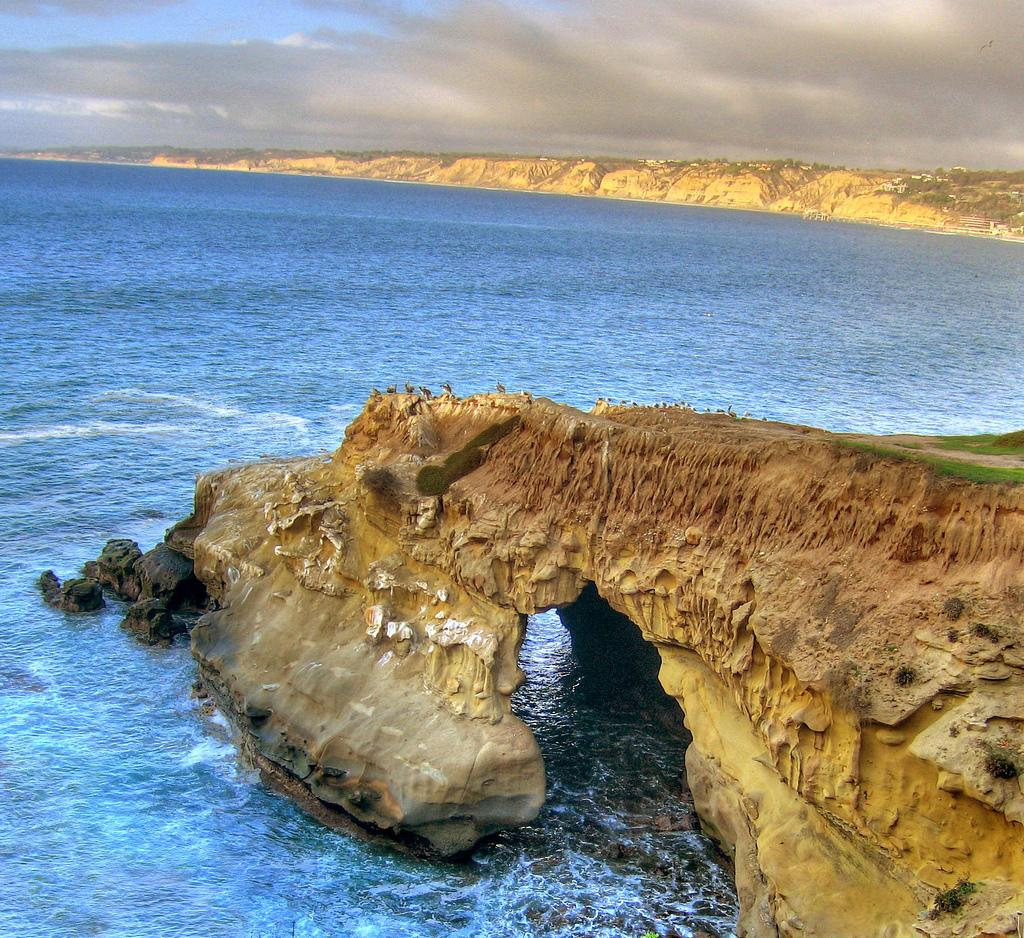
\includegraphics[width = 0.45\textwidth]{imgs/cove_full.jpg}
    \caption{Full Image of La Jolla Cove}
    \label{fig:prob1-afull}
\end{figure}

We break this down into four sections:

\begin{figure}[H]
    \centering
    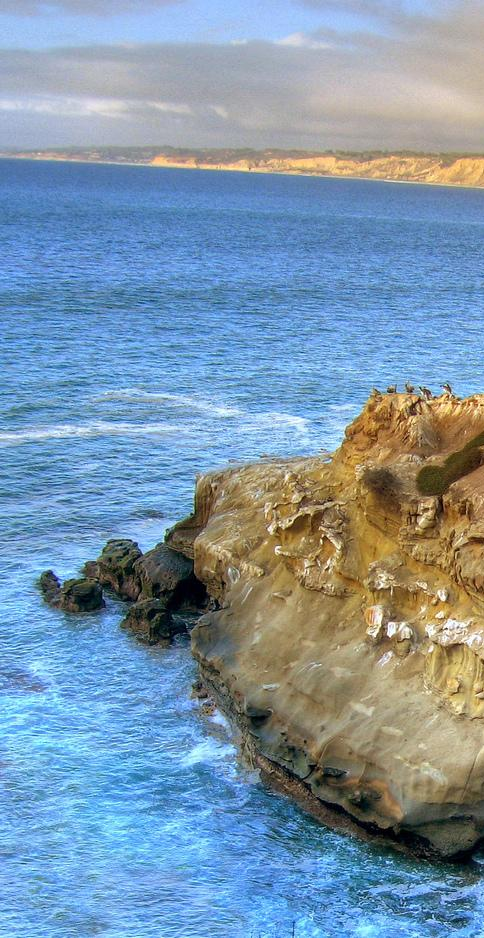
\includegraphics[width = 0.45\textwidth]{imgs/cove_left.png}
    \caption{Left side of the cove}
    \label{fig:prob1-aleft}
\end{figure}

\begin{figure}[H]
    \centering
    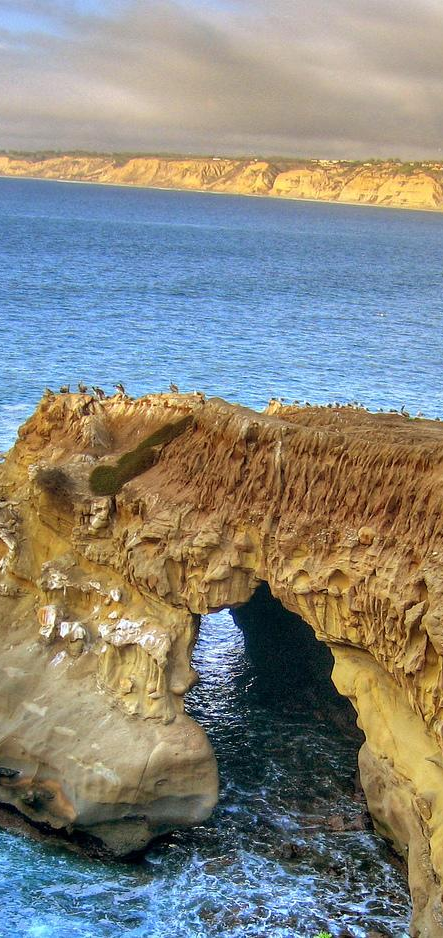
\includegraphics[width = 0.45\textwidth]{imgs/cove_middle.png}
    \caption{Middle of the cove}
    \label{fig:prob1-amiddle}
\end{figure}

\begin{figure}[H]
    \centering
    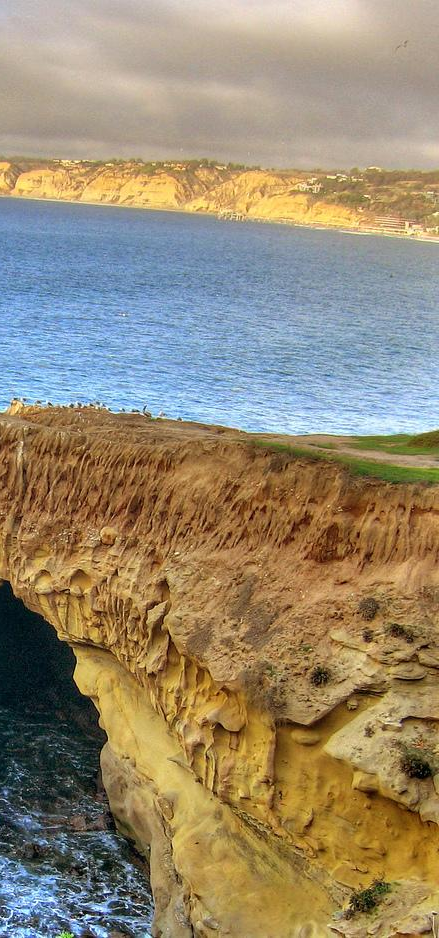
\includegraphics[width = 0.45\textwidth]{imgs/cove_right.png}
    \caption{Right side of the cove}
    \label{fig:prob1-aright}
\end{figure}

\subsection*{B}

Here we identify a series of features across the different sections, and try to match features across the features:

\begin{figure}[H]
    \centering
    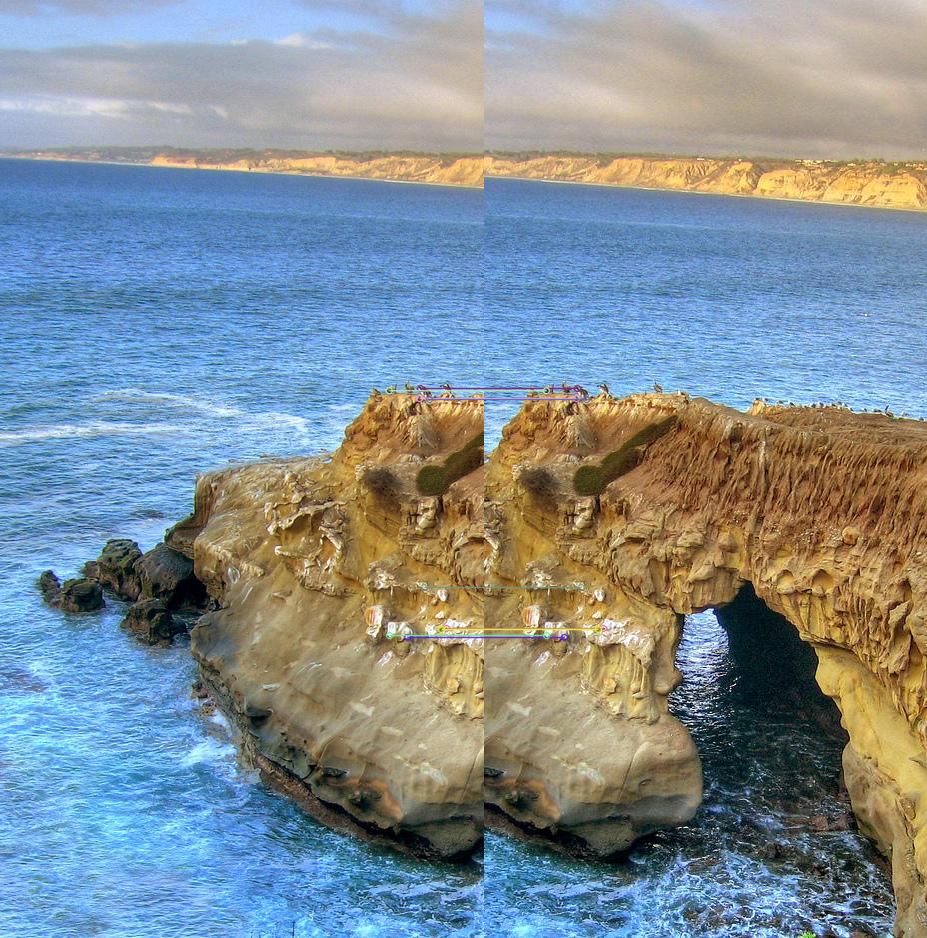
\includegraphics[width = 0.75\textwidth]{imgs/left-middle-matches.png}
    \caption{Left/Middle}
    \label{fig:prob1-b-left-middle}
\end{figure}

\begin{figure}[H]
    \centering
    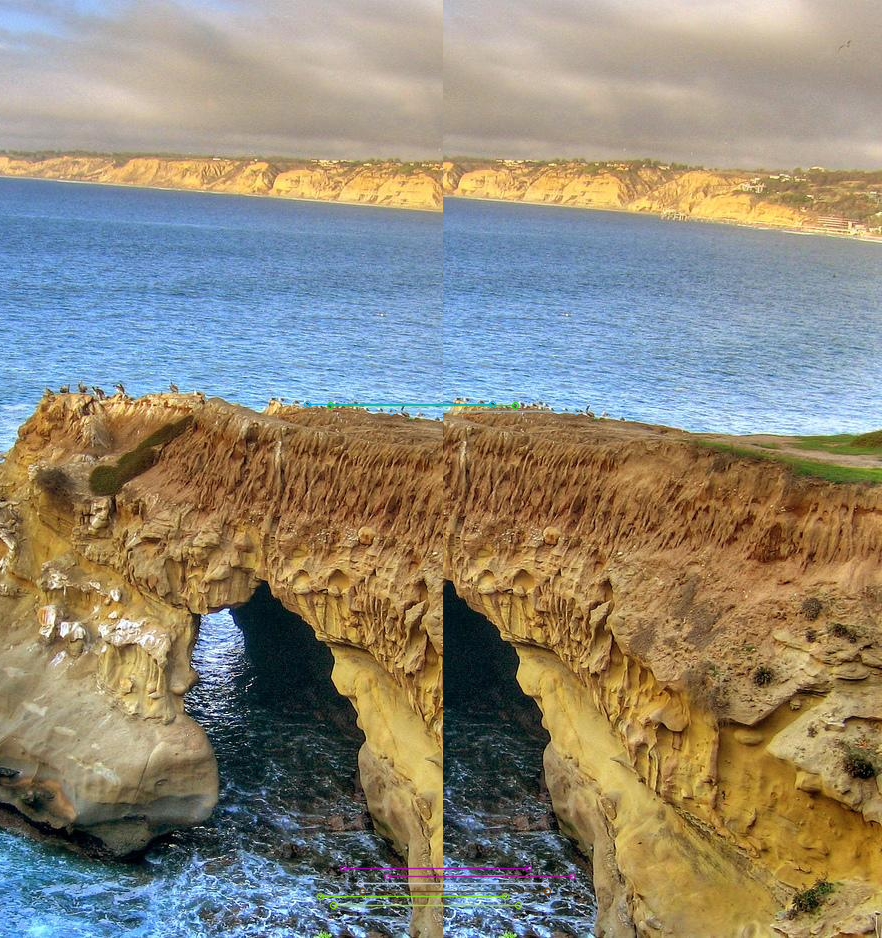
\includegraphics[width = 0.85\textwidth]{imgs/middle-right-matches.png}
    \caption{Middle/Right}
    \label{fig:prob1-b-middle-right}
\end{figure}

\subsection*{C}

Here we are asked to provide a global translation for each image. First, we grab the match results of our pairs - left/middle and middle/right. We assumed here that the left side is situated correctly, which for our side means a translation of $\textbf{[0]}$.

In our code within $problem1.py$, we iterate through the existing points and calcultae the average global translation for each pair. To this end, our software spits out two global translations. For left/middle it resulted in a translation of $(x,y)=(-326,0)$ and for right/middle $(x,y)=(-258,0)$. This makes sense, as how I cut the image was straight cutting the image into sections, suggesting a straight $x$ oriented translation would be all that's required.

\subsection*{D}

To get to the final matching, we will pair the left and middle sides, then feature check the resulting image against the right image.

\begin{figure}[H]
    \centering
    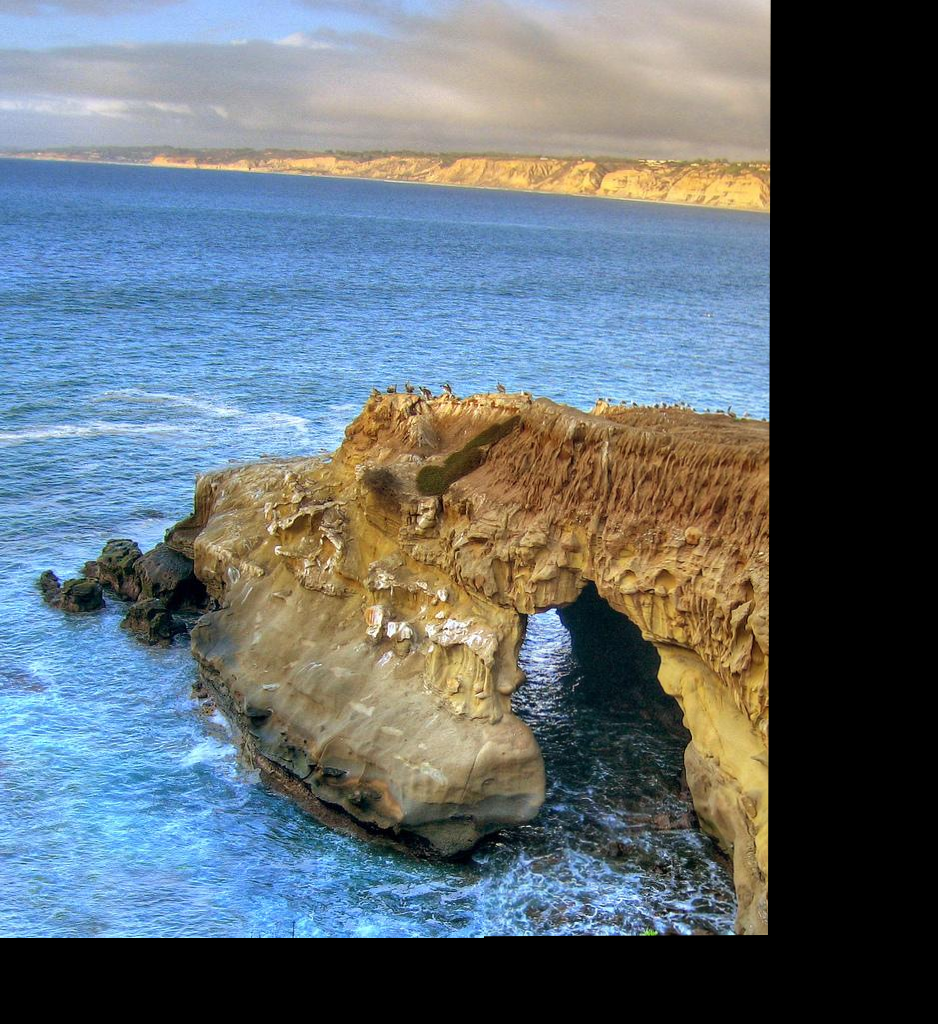
\includegraphics[width = 0.75\textwidth]{imgs/left_middle_match.png}
    \caption{Left/Middle pairing}
    \label{fig:prob1-d-left-middle}
\end{figure}

Then we compare this result against the right side:

\begin{figure}[H]
    \centering
    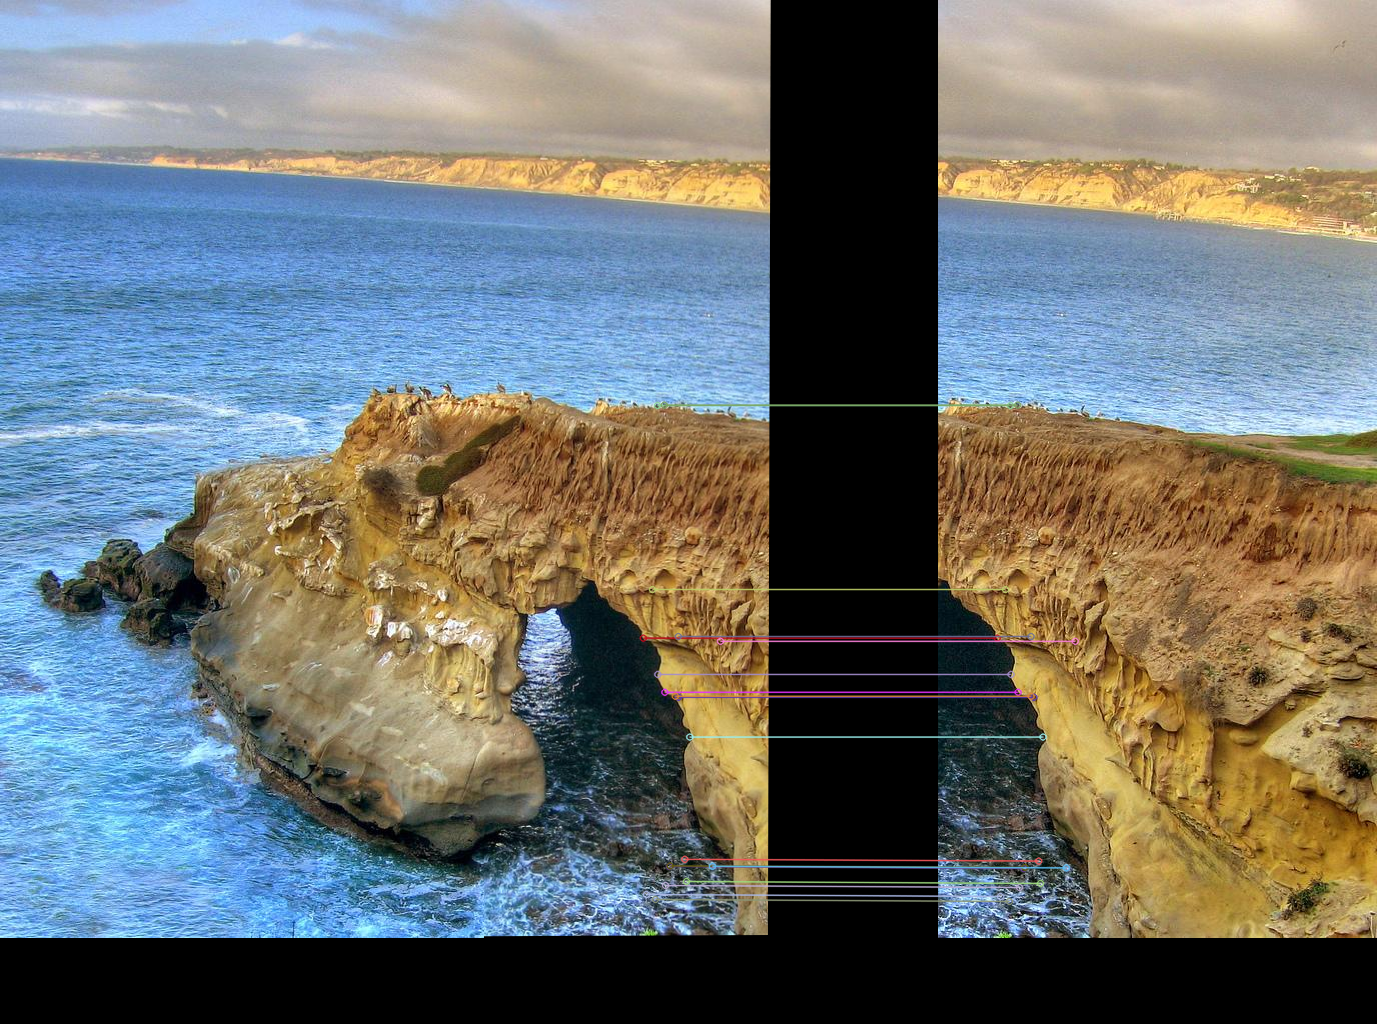
\includegraphics[width = 0.75\textwidth]{imgs/left_middle_match_right.png}
    \caption{Left/Middle - Right Matches}
    \label{fig:prob1-d-leftmiddle-right-matches}
\end{figure}

This leads us to the final output of:

\begin{figure}[H]
    \centering
    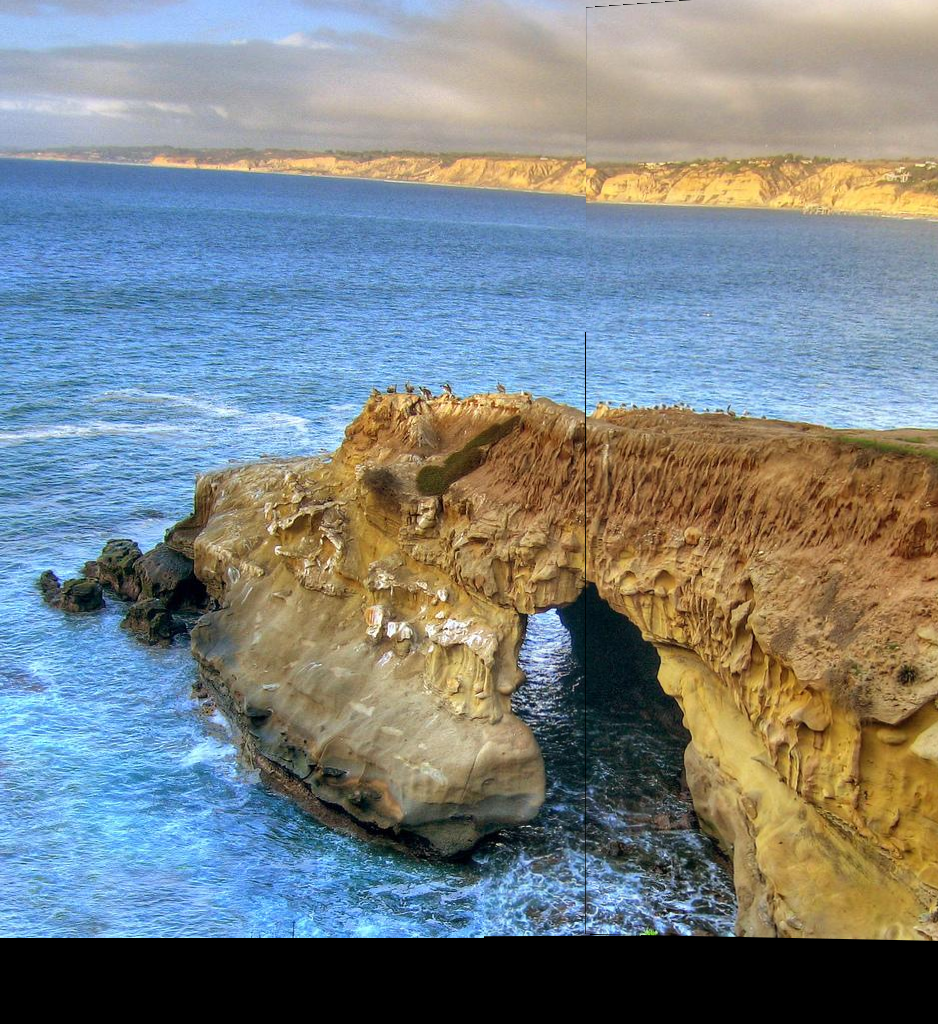
\includegraphics[width = 0.75\textwidth]{imgs/combined_full.png}
    \caption{Fully Combined}
    \label{fig:prob1-d-full-combined}
\end{figure}

\section*{Problem 2}

Here we are presented with two images, seen below:

\begin{figure}[H]
    \centering
    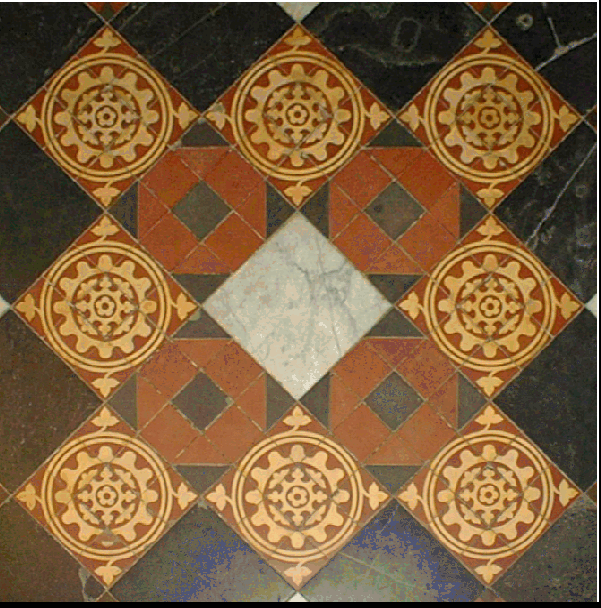
\includegraphics[width = 0.45\textwidth]{imgs/2-1.png}
    \caption{Image 1}
    \label{fig:prob2-1}
\end{figure}

\begin{figure}[H]
    \centering
    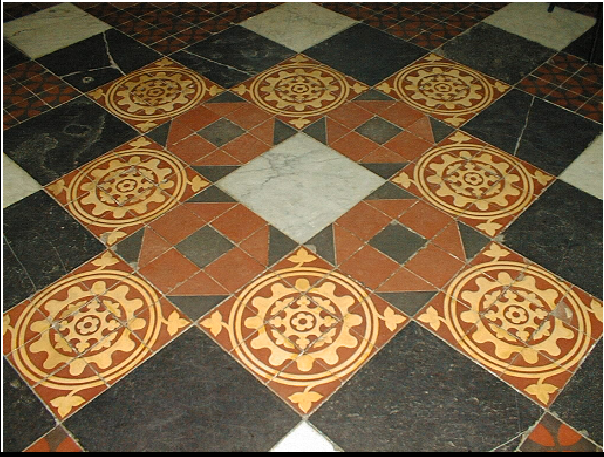
\includegraphics[width = 0.45\textwidth]{imgs/2-2.png}
    \caption{Image 2}
    \label{fig:prob2-2}
\end{figure}

\subsection*{A}

First we pick equivalent spots, tracking them, across the images to try and create a perspective morph. First, our points:

\begin{figure}[H]
    \centering
    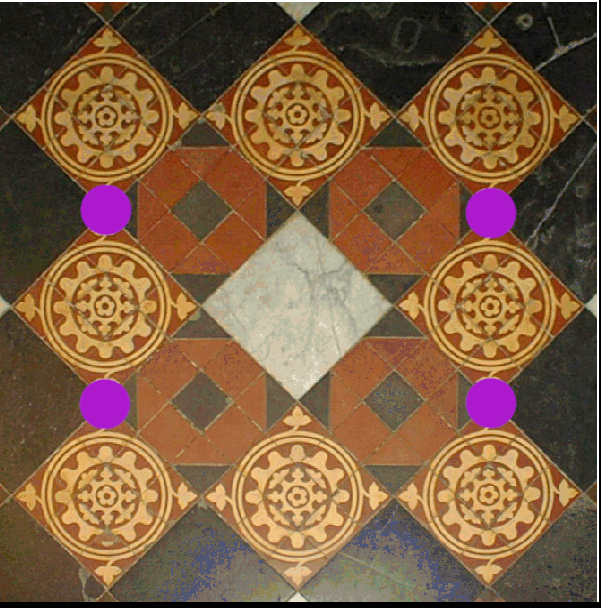
\includegraphics[width = 0.45\textwidth]{imgs/2-1-dots.png}
    \caption{Image 1}
    \label{fig:prob2-1a}
\end{figure}

\begin{figure}[H]
    \centering
    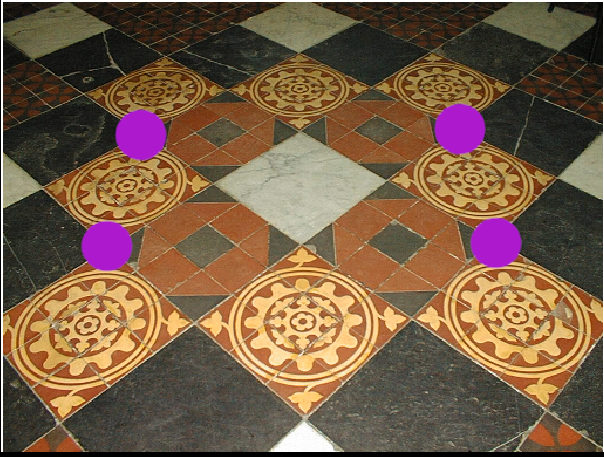
\includegraphics[width = 0.45\textwidth]{imgs/2-2-dots.png}
    \caption{Image 2}
    \label{fig:prob2-1b}
\end{figure}


Our points, as follows:

\begin{equation}
    \begin{tabular}{ | c | c | c | c | c | }
        \hline
        Point & $x_s$ & $y_s$ & $x_d$ & $x_d$\\
        \hline
        1 & 105 & 210 & 140 & 135 \\
        \hline
        2 & 105 & 404 & 107 & 246 \\
        \hline
        3 & 490 & 210 & 460 & 130 \\
        \hline
        4 & 420 & 210 & 496 & 246 \\
        \hline
    \end{tabular}
\end{equation}

\subsection*{B}

We now hope to calculate the homography matrix. To do this we must solve the following:

\begin{equation}
    \begin{bmatrix}
        x^s \\ y^s \\ 1
    \end{bmatrix} = \begin{bmatrix}
        1+h_{11} & h_{12} + h_{13} \\
        h_{21} & 1+h_{22} & h_{23} \\
        h_{31} & h_{32} & 1\\
    \end{bmatrix} =
    \begin{bmatrix}
        x^d \\ y^d \\ 1
    \end{bmatrix}
\end{equation}

To solve for $h$, we can solve it using the following equation:

\begin{equation}
    A = 
    \begin{bmatrix}
        x_s^1 & y_s^1 & 1 & 0 & 0 & 0 & -x_d^1 x_s^1 & -x_d^1 y_s^1 & -x_d^1 \\
        0 & 0 & 0 &  x_s^1 & y_s^1 & 1 & -y_d^1 x_s^1 &-y_d^1 y_s^1 & -y_d^1 \\
        \vdots &\vdots &\vdots &\vdots &\vdots &\vdots &\vdots &\vdots &\vdots \\
        x_s^4 & y_s^4 & 1 & 0 & 0 & 0 & -x_d^4 x_s^4 & -x_d^4 y_s^4 & -x_d^4 \\
        0 & 0 & 0 &  x_s^4 & y_s^4 & 1 & -y_d^4 x_s^4 &-y_d^4 y_s^4 & -y_d^4 \\
    \end{bmatrix}
\end{equation}

\begin{equation}
    h = \begin{bmatrix}
        h_{11} \\
        h_{12} \\
        h_{13} \\
        h_{21} \\
        h_{22} \\
        h_{23} \\
        h_{31} \\
        h_{32} \\
        h_{33} \\
    \end{bmatrix}
\end{equation}

And with these we can then solve it by setting it equal to :

\begin{equation}
    Ah = \begin{bmatrix}
        0 \\ 0 \\ 0 \\ 0 \\ 0 \\ 0 \\ 0 \\ 1
    \end{bmatrix}
\end{equation}

...from this we can solve that $h$ is equal to:

\begin{equation}
    h = \begin{bmatrix}
        h_{11} \\
        h_{12} \\
        h_{13} \\
        h_{21} \\
        h_{22} \\
        h_{23} \\
        h_{31} \\
        h_{32} \\
        h_{33} \\
    \end{bmatrix} = \begin{bmatrix}
        0.0 \\
        0.0042 \\
        1.536 \\
        -0.0058 \\
        0.0147 \\
        -1.757 \\
        0.0 \\
        0.0 \\
        0
    \end{bmatrix}
\end{equation}

So when we apply it to the homogaphy matrix as we listed above in \textbf{2}:

\begin{equation}
    \begin{bmatrix}
        1 & 0.0042 & 1.536 \\
        -0.0058 & 1.0147 & -1.757 \\
        0.0 & 0.0 & 1\\
    \end{bmatrix}
\end{equation}

The work for this can be found below:

\begin{verbatim}
%xs ys 1 0 0 0 -xd.xs -xd.ys -xd;
%0  0  0 xs ys 1 -yd.xs -yd.ys -yd;

A = [
    % first point - (105, 210) -> (140, 135)
    105 210 1 0 0 0 -140*105 -140*210 -140;
    0   0   0   105 210 1 -135*105 -135*210 -135;

    %second point - (105, 404) -> (107, 246)
    105 404 1 0 0 0 -107*105 -107*404 -107;
    0   0   0 105 404 1 -246*105 -246*404 -246;

    %third point - (490, 210) -> (460, 130)
    490 210 1 0 0 0 -460*490 -460*210 -460;
    0   0   0 490 210 1 -130*490 -130*210 -130;

    %fourth point - (420, 210) -> (496,246)
    420 210 1 0 0 0 -496*420 -496*210 -496;
    0   0   0 420 210 1 -246*420 -246*210 -246;
]

syms h11 h12 h13 h21 h22 h23 h31 h32 h33

h = [h11; h12; h13; h21; h22; h23; h31; h32; h33;]

solve(A*h==[0; 0; 0; 0; 0; 0; 0; 1;], h)
  
\end{verbatim}

\end{document}